% !TeX program = xelatex
\documentclass[12pt,a4paper]{article}
\usepackage{fontspec}
\setmainfont{Times New Roman}[Path=C:/Windows/Fonts/,UprightFont=times.ttf,BoldFont=timesbd.ttf,ItalicFont=timesi.ttf,BoldItalicFont=timesbi.ttf]
\usepackage{amsmath,amssymb,amsfonts}
\usepackage[left=1.5cm,right=1.5cm,top=1.4cm,bottom=1.6cm,headheight=17pt]{geometry}
\usepackage{enumitem,array,graphicx,tikz,fancyhdr,needspace}
\usetikzlibrary{arrows.meta,calc,patterns}
% Sửa số đề và số trang đề thực tế sau khi biên dịch/tách PDF.
\newcommand{\soDe}{11}
\newcommand{\soTrangDe}{4}
\newcommand{\maDe}{\ifnum\soDe<1000 0\fi\ifnum\soDe<100 0\fi\ifnum\soDe<10 0\fi\soDe}
\pagestyle{fancy}
\fancyhf{}
\lhead{\small\textbf{ÔN TẬP GIỮA KÌ I}}
\rhead{\small\textit{Biên soạn: Dương Gia Bảo}}
\rfoot{\small Trang \thepage/\soTrangDe\ - Mã đề: \maDe}
\renewcommand{\headrulewidth}{0.4pt}
\fancypagestyle{answers}{\rfoot{\small Trang \thepage\ - Mã đề: \maDe}}
\fancypagestyle{firstpage}{\fancyhead{}\renewcommand{\headrulewidth}{0pt}}
\setlength{\parindent}{0pt}
\setlength{\parskip}{2.5pt}
\setlength{\emergencystretch}{1em}
\setlist[enumerate,1]{label=\textbf{Câu \arabic*:},leftmargin=*,itemsep=5pt,topsep=2pt}
\setlist[enumerate,2]{label=\alph*),leftmargin=*,itemsep=2pt,topsep=2pt}
\newcommand{\bonpa}[4]{\par\nobreak\smallskip\nobreak\noindent
\begin{tabular}{@{}p{0.47\linewidth}p{0.47\linewidth}@{}}
\textbf{A.} #1 & \textbf{B.} #2\\[8pt]
\textbf{C.} #3 & \textbf{D.} #4\end{tabular}}
\newcommand{\loigiai}[1]{\par\medskip\Needspace{4\baselineskip}\noindent\textbf{#1}\par\nobreak}
\newcommand{\otraloi}{\par\nobreak\smallskip\noindent\textit{Trả lời:}\quad\fbox{\rule{0pt}{11pt}\makebox[0.3cm]{}}\,\fbox{\rule{0pt}{11pt}\makebox[0.3cm]{}}\,\fbox{\rule{0pt}{11pt}\makebox[0.3cm]{}}\,\fbox{\rule{0pt}{11pt}\makebox[0.3cm]{}}}
\begin{document}
\thispagestyle{firstpage}
\noindent
\begin{minipage}[t]{0.35\textwidth}
    \centering
    {\fontsize{13}{15}\selectfont\textbf{ÔN TẬP GIỮA KÌ I}}\\[4pt]
    \textit{Biên soạn: Dương Gia Bảo}\\[5pt]
    \setlength{\fboxrule}{0.8pt}%
    \setlength{\fboxsep}{4pt}%
    \fbox{\begin{minipage}{0.83\linewidth}
        \centering
        {\fontsize{13}{15}\selectfont\textbf{ĐỀ ÔN TẬP}\\[2pt]\textbf{CHƯƠNG I VÀ II}}\\[4pt]
        \textit{(Đề thi gồm có \ifnum\soTrangDe<10 0\fi\soTrangDe\ trang)}
    \end{minipage}}
\end{minipage}\hfill
\begin{minipage}[t]{0.63\textwidth}
    \centering
    {\fontsize{13}{15}\selectfont\textbf{ÔN TẬP KIỂM TRA GIỮA KÌ I}\\[2pt]
    \textbf{NĂM HỌC 2026 - 2027}}\\[5pt]
    {\fontsize{14}{16}\selectfont\textbf{Môn: TOÁN - Lớp 12 (ĐỀ SỐ \soDe)}}\\[4pt]
    {\fontsize{11.5}{13}\selectfont\textit{Thời gian làm bài: 90 phút, không kể thời gian giao đề}}\\[5pt]
    \setlength{\fboxrule}{0.8pt}%
    \setlength{\fboxsep}{5pt}%
    \fbox{\makebox[3cm]{\fontsize{14}{16}\selectfont\textbf{Mã đề: \maDe}}}
\end{minipage}
\par\vspace{2pt}
\hrule height 0.6pt
\vspace{3pt}
\noindent\textit{Họ và tên học sinh:}\dotfill\hspace{1cm}\textit{Lớp:}\makebox[3.5cm]{\dotfill}
\par\vspace{2pt}
\hrule height 0.6pt
\vspace{3pt}

\section*{\large PHẦN I. Câu trắc nghiệm nhiều phương án lựa chọn}
\textit{Thí sinh trả lời từ câu 1 đến câu 12. Mỗi câu chỉ chọn một phương án.}
\begin{enumerate}
\item Cho hàm số $y=x^3-3x^2-9x+2$. Hàm số đã cho nghịch biến trên khoảng nào dưới đây?
\bonpa{$(-1;3)$.}{$(-\infty;-1)$.}{$(3;+\infty)$.}{$(0;4)$.}

\item Cho hàm số $y=-x^3+3x^2+9x-1$. Điểm cực đại của hàm số đã cho là
\bonpa{$x=-1$.}{$x=3$.}{$x=26$.}{$x=-6$.}

\item Giá trị lớn nhất của hàm số $f(x)=\dfrac{2x-1}{x+1}$ trên đoạn $[0;3]$ bằng
\bonpa{$-1$.}{$1$.}{$\dfrac{5}{4}$.}{$2$.}

\item Đường tiệm cận đứng của đồ thị hàm số $y=\dfrac{3x+2}{x-2}$ là đường thẳng có phương trình
\bonpa{$y=3$.}{$x=-2$.}{$y=-1$.}{$x=2$.}

\item Đường tiệm cận xiên của đồ thị hàm số $y=\dfrac{2x^2+3x-1}{x+1}$ có phương trình là
\bonpa{$y=2x+1$.}{$y=2x-1$.}{$y=x+1$.}{$y=2x+3$.}

\item Đường cong trong hình vẽ bên là đồ thị của hàm số nào dưới đây?
\par\nobreak\smallskip
\begin{minipage}[c]{0.62\linewidth}
\bonpa{$y=\dfrac{x^2-x+1}{x-1}$.}{$y=\dfrac{x^2-2x+2}{x-1}$.}{$y=\dfrac{x^2+2x-2}{x+1}$.}{$y=\dfrac{x^2-3x+3}{x-2}$.}
\end{minipage}\hfill
\begin{minipage}[c]{0.36\linewidth}\centering
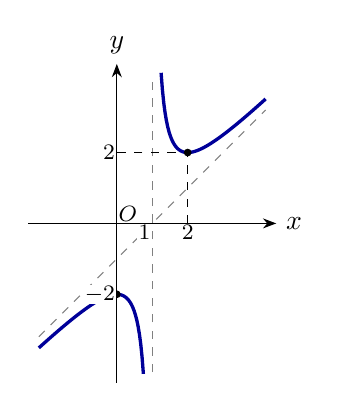
\begin{tikzpicture}[x=0.45cm,y=0.45cm,>=Stealth]
\draw[->] (-2.5,0)--(4.5,0) node[right] {$x$};
\draw[->] (0,-4.5)--(0,4.5) node[above] {$y$};
\draw[dashed,gray] (1,-4.2)--(1,4.2);
\draw[dashed,gray] (-2.2,-3.2)--(4.2,3.2);
\draw[very thick,blue!60!black,domain=-2.2:0.75,samples=80] plot (\x,{(\x*\x-2*\x+2)/(\x-1)});
\draw[very thick,blue!60!black,domain=1.25:4.2,samples=80] plot (\x,{(\x*\x-2*\x+2)/(\x-1)});
\draw[dashed] (2,0)--(2,2)--(0,2);
\fill (0,-2) circle (1.4pt);
\fill (2,2) circle (1.4pt);
\node[above right,fill=white,inner sep=0.5pt] at (0,0) {\footnotesize $O$};
\node[below left,fill=white,inner sep=0.5pt] at (1,0) {\footnotesize $1$};
\node[below,fill=white,inner sep=0.5pt] at (2,0) {\footnotesize $2$};
\node[left,fill=white,inner sep=0.5pt] at (0,-2) {\footnotesize $-2$};
\node[left,fill=white,inner sep=0.5pt] at (0,2) {\footnotesize $2$};
\end{tikzpicture}
\end{minipage}
\end{enumerate}

\newpage
\begin{enumerate}[start=7]
\item Một xưởng may đồng phục bán mỗi sản phẩm với giá $p$ nghìn đồng ($50\le p\le 250$). Số lượng sản phẩm bán ra theo giá $p$ là $D(p)=600-2p$. Doanh thu từ việc bán sản phẩm là $R(p)=p\cdot D(p)=600p-2p^2$ (nghìn đồng). Để doanh thu đạt giá trị lớn nhất thì giá bán $p$ bằng bao nhiêu nghìn đồng?
\bonpa{$100$.}{$120$.}{$150$.}{$200$.}

\item Cho hình hộp $ABCD.A'B'C'D'$. Vectơ tổng $\vec{AB}+\vec{AD}+\vec{AA'}$ bằng vectơ nào dưới đây?
\bonpa{$\vec{AC}$.}{$\vec{CA'}$.}{$\vec{BD'}$.}{$\vec{AC'}$.}

\item Trong không gian $Oxyz$, cho hai điểm $A(2;-1;3)$ và $B(4;3;-1)$. Tọa độ trung điểm $M$ của đoạn thẳng $AB$ là
\bonpa{$(3;1;1)$.}{$(6;2;2)$.}{$(1;2;-2)$.}{$(2;4;-4)$.}

\item Trong không gian $Oxyz$, cho hai vectơ $\vec{a}=(1;-2;3)$ và $\vec{b}=(-2;1;1)$. Tọa độ của vectơ $\vec{u}=2\vec{a}+\vec{b}$ là
\bonpa{$(-1;-1;4)$.}{$(0;-3;7)$.}{$(0;-1;7)$.}{$(4;-5;5)$.}

\item Trong không gian $Oxyz$, cho hai vectơ $\vec{u}=(2;-1;2)$ và $\vec{v}=(1;2;-2)$. Tích vô hướng $\vec{u}\cdot\vec{v}$ bằng
\bonpa{$4$.}{$0$.}{$-4$.}{$-2$.}

\item Trong không gian $Oxyz$, cho hai điểm $A(1;2;-1)$ và $B(3;0;0)$. Độ dài đoạn thẳng $AB$ bằng
\bonpa{$\sqrt{5}$.}{$9$.}{$\sqrt{7}$.}{$3$.}
\end{enumerate}

\vspace{3pt}
\section*{\large PHẦN II. Câu trắc nghiệm đúng hoặc sai}
\textit{Thí sinh trả lời từ câu 1 đến câu 4. Trong mỗi ý a), b), c), d) ở mỗi câu, thí sinh chọn đúng hoặc sai.}
\begin{enumerate}
\item Cho hàm số $y=f(x)=\dfrac{x^2-3x+3}{x-1}$.
\begin{enumerate}
\item Tập xác định của hàm số là $D=\mathbb{R}\setminus\{1\}$.
\item Đạo hàm của hàm số là $f'(x)=\dfrac{x^2-2x}{(x-1)^2}$ với mọi $x\ne 1$.
\item Đồ thị hàm số có đường tiệm cận xiên là đường thẳng $y=x+2$.
\item Khoảng cách giữa hai điểm cực trị của đồ thị hàm số bằng $2\sqrt{5}$.
\end{enumerate}
\end{enumerate}

\newpage
\begin{enumerate}[start=2]
\item Trong một phòng thí nghiệm sinh học, nồng độ khí $\text{CO}_2$ trong phòng thay đổi theo thời gian $t$ (giờ, $t\ge 0$) kể từ khi bắt đầu thí nghiệm và được mô hình hóa bởi hàm số $C(t)=\dfrac{400t^2+200}{t^2+1}$ (đơn vị: ppm).
\begin{enumerate}
\item Nồng độ khí $\text{CO}_2$ trong phòng tại thời điểm ban đầu ($t=0$) là $200\text{ ppm}$.
\item Nồng độ khí $\text{CO}_2$ trong phòng luôn tăng trong suốt quá trình thí nghiệm ($t>0$).
\item Sau $3$ giờ kể từ khi bắt đầu thí nghiệm, nồng độ khí $\text{CO}_2$ trong phòng đạt $380\text{ ppm}$.
\item Khi thời gian $t$ kéo dài vô hạn ($t\to+\infty$), nồng độ khí $\text{CO}_2$ trong phòng sẽ vượt quá mức $450\text{ ppm}$.
\end{enumerate}

\item Trong không gian $Oxyz$, cho ba điểm $A(1;1;2)$, $B(3;2;0)$ và $C(-1;3;5)$.
\begin{enumerate}
\item Tọa độ của vectơ $\vec{AB}$ là $\vec{AB}=(2;1;-2)$ và độ dài đoạn thẳng $AB$ bằng $3$.
\item Trọng tâm $G$ của tam giác $ABC$ có tọa độ là $G\left(1;2;\dfrac{7}{3}\right)$.
\item Tọa độ điểm $D$ để tứ giác $ABCD$ là hình bình hành là $D(-3;2;7)$.
\item Góc giữa hai vectơ $\vec{AB}$ và $\vec{AC}$ là một góc nhọn.
\end{enumerate}

\item Một vật nặng có trọng lượng $P=180\text{ N}$ được giữ cân bằng trong không gian $Oxyz$ bởi ba sợi dây cáp mảnh, không dãn. Ba đầu dây phía trên được gắn cố định vào trần nhà nằm ngang (mặt phẳng $Oxy$) tại ba điểm $A(-6;-2;0)$, $B(6;-2;0)$ và $C(0;4;0)$, còn ba đầu dây phía dưới cùng được buộc vào móc treo vật tại điểm $D(0;0;-3)$ (đơn vị đo trên các trục là mét, trục $Oz$ hướng thẳng đứng lên trên). Trọng lực tác dụng lên vật là $\vec{P}=(0;0;-180)\text{ N}$. Lực căng tác dụng lên các sợi dây lần lượt là $\vec{F}_1$ (dọc theo $\vec{DA}$), $\vec{F}_2$ (dọc theo $\vec{DB}$) và $\vec{F}_3$ (dọc theo $\vec{DC}$).
\begin{enumerate}
\item Độ dài của sợi dây cáp nối từ móc treo $D$ đến điểm cố định $C$ bằng $5\text{ m}$.
\item Vì vật ở trạng thái cân bằng nên ta có hệ thức vectơ $\vec{F}_1+\vec{F}_2+\vec{F}_3+\vec{P}=\vec{0}$.
\item Lực căng tác dụng lên hai sợi dây treo $DA$ và $DB$ có độ lớn bằng nhau và bằng $140\text{ N}$.
\item Lực căng tác dụng lên sợi dây treo $DC$ có độ lớn bằng $120\text{ N}$.
\end{enumerate}
\end{enumerate}

\vspace{3pt}
\section*{\large PHẦN III. Câu trắc nghiệm trả lời ngắn}
\textit{Thí sinh trả lời từ câu 1 đến câu 6. Mỗi câu trả lời đúng thí sinh được 0,5 điểm.}
\begin{enumerate}
\item Tìm số giá trị nguyên của tham số $m\in[-10;10]$ để hàm số $y=\dfrac{1}{3}x^3-mx^2+(2m+8)x-2027$ đồng biến trên khoảng $(-\infty;+\infty)$.
\otraloi

\item Trong không gian $Oxyz$, cho hình hộp $ABCD.A'B'C'D'$ có tọa độ các đỉnh $A(1;2;-1)$, $B(3;1;2)$, $D(2;4;1)$ và $A'(3;5;0)$. Tìm tọa độ đỉnh $C'(x;y;z)$, sau đó tính tổng $S=x+y+z$.
\otraloi
\end{enumerate}

\newpage
\begin{enumerate}[start=3]
\item Cho hàm số $y=\dfrac{x^2+mx+4}{x+2}$ ($m$ là tham số thực). Có bao nhiêu giá trị nguyên của tham số $m\in[-5;5]$ để đồ thị hàm số có hai điểm cực trị nằm về hai phía của trục tung?
\otraloi

\item Trong không gian $Oxyz$ (đơn vị trên các trục là mét), có hai thiết bị bay không người lái (drone) $A$ và $B$ đang bay thử nghiệm. Tại thời điểm $t$ giây ($t\ge 0$), vị trí của drone $A$ là $A(2+t;10+2t;1+3t)$ và vị trí của drone $B$ là $B(2t;6t+5;11)$. Khoảng cách ngắn nhất giữa hai drone trong quá trình bay bằng bao nhiêu mét?
\otraloi

\item Từ một tấm tôn hình vuông cạnh $60\text{ cm}$, người ta cắt bỏ bốn hình vuông bằng nhau ở bốn góc, mỗi hình vuông có cạnh bằng $x\text{ cm}$, rồi gập các mép lại để tạo thành một chiếc hộp hình hộp chữ nhật không có nắp (hình vẽ minh họa). Hỏi thể tích lớn nhất của chiếc hộp bằng bao nhiêu đềximét khối ($\text{dm}^3$)?
\begin{center}
\begin{tikzpicture}[x=0.55cm,y=0.55cm,>=Stealth]
% Flat sheet
\draw[thick] (0,0) rectangle (5,5);
\fill[gray!30] (0,0) rectangle (1,1);
\fill[gray!30] (4,0) rectangle (5,1);
\fill[gray!30] (0,4) rectangle (1,5);
\fill[gray!30] (4,4) rectangle (5,5);
\draw[dashed] (1,0)--(1,5) (4,0)--(4,5) (0,1)--(5,1) (0,4)--(5,4);
\draw[<->] (0,-0.5)--(5,-0.5) node[midway,below] {\footnotesize $60\text{ cm}$};
\draw[<->] (-0.5,0)--(-0.5,5) node[midway,left] {\footnotesize $60\text{ cm}$};
\draw[<->] (0,1.2)--(1,1.2) node[midway,above] {\footnotesize $x$};
\draw[<->] (1.2,0)--(1.2,1) node[midway,right] {\footnotesize $x$};

% Arrow
\draw[->,very thick,gray!70] (6,2.5)--(7.5,2.5) node[midway,above] {\footnotesize Gập hộp};

% Folded 3D box
\begin{scope}[shift={(8.5,0.8)}]
\coordinate (A) at (0,0);
\coordinate (B) at (3.2,0);
\coordinate (C) at (4.4,1.1);
\coordinate (D) at (1.2,1.1);
\coordinate (A1) at (0,1.5);
\coordinate (B1) at (3.2,1.5);
\coordinate (C1) at (4.4,2.6);
\coordinate (D1) at (1.2,2.6);

\draw[dashed,thick,gray!80] (A)--(D)--(C);
\draw[dashed,thick,gray!80] (D)--(D1);

\fill[blue!5,opacity=0.6] (A)--(B)--(C)--(D)--cycle;
\fill[blue!10,opacity=0.4] (A)--(B)--(B1)--(A1)--cycle;
\fill[blue!15,opacity=0.4] (B)--(C)--(C1)--(B1)--cycle;

\draw[thick] (A)--(B)--(C);
\draw[thick] (A1)--(B1)--(C1)--(D1)--cycle;
\draw[thick] (A)--(A1) (B)--(B1) (C)--(C1);

\draw[<->] (0,-0.4)--(3.2,-0.4) node[midway,below] {\footnotesize $60-2x$};
\draw[<->] (-0.4,0)--(-0.4,1.5) node[midway,left] {\footnotesize $x$};
\end{scope}
\end{tikzpicture}
\par\smallskip{\footnotesize\textit{Tấm tôn cắt 4 góc và chiếc hộp hình hộp chữ nhật không nắp.}}
\end{center}
\otraloi

\item Một trạm biến áp trên một hòn đảo $A$ cần kéo đường dây cáp điện nối vào nhà máy điện $B$ nằm trên đất liền dọc theo bờ biển thẳng. Khoảng cách từ đảo $A$ đến bờ biển là $AH=6\text{ km}$ ($H$ là hình chiếu vuông góc của $A$ lên bờ biển). Khoảng cách từ $H$ đến nhà máy $B$ dọc theo bờ biển là $HB=12\text{ km}$. Người ta dự định kéo đường dây cáp gồm hai đoạn: đoạn cáp ngầm đi dưới biển từ trạm đảo $A$ đến điểm $C$ trên bờ biển ($C$ nằm giữa $H$ và $B$), và đoạn cáp trên bờ chạy dọc theo bờ biển từ $C$ đến nhà máy $B$ (hình vẽ minh họa). Biết chi phí lắp đặt cáp ngầm dưới biển là $100$ triệu đồng/km, chi phí lắp đặt cáp trên bờ là $60$ triệu đồng/km. Tổng chi phí lắp đặt nhỏ nhất của toàn bộ đường cáp bằng bao nhiêu triệu đồng?
\begin{center}
\begin{tikzpicture}[x=0.70cm,y=0.70cm,>=Stealth]
\draw[thick,blue!50!gray] (-0.5,0)--(13.0,0) node[above,black] {\footnotesize Đường bờ biển};
\fill[cyan!10] (-0.5,-2.8) rectangle (13.0,0);
\node at (5.5,-2.0) {\textit{\footnotesize Biển}};
\node at (5.5,0.7) {\textit{\footnotesize Đất liền}};

\coordinate (H) at (1.0,0);
\coordinate (C) at (5.5,0);
\coordinate (B) at (12.0,0);
\coordinate (A) at (1.0,-2.5);

\fill (H) circle (2pt) node[above] {$H$};
\fill (C) circle (2pt) node[above] {$C$};
\fill (B) circle (2pt) node[above] {$B$ (Nhà máy)};
\fill (A) circle (2pt) node[below] {$A$ (Đảo)};

\draw[dashed] (A)--(H);
\draw (1.0,-0.3)--(1.3,-0.3)--(1.3,0);
\draw[line width=1.5pt,red!80!black] (A)--(C) node[midway,below right] {\footnotesize Cáp ngầm};
\draw[line width=1.5pt,orange!80!black] (C)--(B) node[midway,above] {\footnotesize Cáp trên bờ};

\draw[<->] (1.0,-0.3)--(5.5,-0.3) node[midway,below] {\footnotesize $x$};
\draw[<->] (0.5,0)--(0.5,-2.5) node[midway,left] {\footnotesize $6\text{ km}$};
\draw[<->] (1.0,0.4)--(12.0,0.4) node[midway,above] {\footnotesize $HB = 12\text{ km}$};
\end{tikzpicture}
\par\smallskip{\footnotesize\textit{Sơ đồ phương án kéo đường cáp từ trạm phát đảo $A$ đến nhà máy $B$.}}
\end{center}
\otraloi
\end{enumerate}
\begin{center}\textbf{---------------- HẾT ----------------}\end{center}

\newpage\pagestyle{answers}
\begin{center}\Large\textbf{BẢNG ĐÁP ÁN TỔNG HỢP}\end{center}
\textbf{Phần I. Trắc nghiệm nhiều phương án lựa chọn}
\begin{center}
\renewcommand{\arraystretch}{1.5}
\begin{tabular}{|c|*{12}{c|}}\hline
Câu & 1&2&3&4&5&6&7&8&9&10&11&12\\\hline
Đáp án & A & B & C & D & A & B & C & D & A & B & C & D \\\hline
\end{tabular}
\end{center}

\textbf{Phần II. Đúng hoặc sai}
\begin{center}
\renewcommand{\arraystretch}{1.4}
\begin{tabular}{|c|c|c|c|c|}\hline
Câu & a) & b) & c) & d)\\\hline
1 & Đ & Đ & S & Đ\\\hline
2 & Đ & Đ & Đ & S\\\hline
3 & Đ & Đ & Đ & S\\\hline
4 & Đ & Đ & Đ & S\\\hline
\end{tabular}
\end{center}

\textbf{Phần III. Trả lời ngắn}
\begin{center}
\renewcommand{\arraystretch}{1.5}
\begin{tabular}{|c|c|c|c|c|c|c|}\hline
Câu & 1 & 2 & 3 & 4 & 5 & 6\\\hline
Đáp án & 7 & 17 & 7 & 5 & 16 & 1200 \\\hline
\end{tabular}
\end{center}

\vspace{0.5cm}
\begin{center}
\large\textbf{HƯỚNG DẪN GIẢI CHI TIẾT}
\end{center}

\section*{PHẦN I}

\loigiai{Câu 1. Chọn A.}
Hàm số đã cho là $y=x^3-3x^2-9x+2$.
Tập xác định: $D=\mathbb{R}$.
Đạo hàm: $y'=3x^2-6x-9=3(x^2-2x-3)=3(x+1)(x-3)$.
Ta có $y'<0 \iff x^2-2x-3 < 0 \iff -1 < x < 3$.
Do đó, hàm số nghịch biến trên khoảng $(-1;3)$.

\loigiai{Câu 2. Chọn B.}
Hàm số đã cho là $y=-x^3+3x^2+9x-1$.
Tập xác định: $D=\mathbb{R}$.
Đạo hàm: $y'=-3x^2+6x+9=-3(x^2-2x-3)=-3(x+1)(x-3)$.
$y'=0 \iff x=-1$ hoặc $x=3$.
Đạo hàm cấp hai: $y''=-6x+6$.
Tại $x=3$: $y''(3)=-6(3)+6=-12<0$, suy ra $x=3$ là điểm cực đại của hàm số.
(Tại $x=-1$: $y''(-1)=12>0$ là điểm cực tiểu của hàm số; giá trị cực đại là $y(3)=26$).

\loigiai{Câu 3. Chọn C.}
Hàm số $f(x)=\dfrac{2x-1}{x+1}$ xác định và liên tục trên đoạn $[0;3]$.
Đạo hàm: $f'(x)=\dfrac{2(1)-(-1)(1)}{(x+1)^2}=\dfrac{3}{(x+1)^2}>0$ với mọi $x\in[0;3]$.
Suy ra hàm số luôn đồng biến trên đoạn $[0;3]$.
Do đó, giá trị lớn nhất của hàm số trên đoạn $[0;3]$ là $\max_{[0;3]} f(x)=f(3)=\dfrac{2(3)-1}{3+1}=\dfrac{5}{4}$.

\loigiai{Câu 4. Chọn D.}
Xét hàm số $y=\dfrac{3x+2}{x-2}$.
Tập xác định: $D=\mathbb{R}\setminus\{2\}$.
Ta có $\lim_{x\to 2^+} \dfrac{3x+2}{x-2}=+\infty$ và $\lim_{x\to 2^-} \dfrac{3x+2}{x-2}=-\infty$.
Do đó, đường thẳng $x=2$ là đường tiệm cận đứng của đồ thị hàm số đã cho.

\loigiai{Câu 5. Chọn A.}
Ta có biểu thức:
$y=\dfrac{2x^2+3x-1}{x+1} = \dfrac{2x(x+1) + (x+1) - 2}{x+1} = 2x+1 - \dfrac{2}{x+1}$.
Mặt khác:
$\lim_{x\to\pm\infty} [y - (2x+1)] = \lim_{x\to\pm\infty} \left(-\dfrac{2}{x+1}\right) = 0$.
Vậy đường thẳng $y=2x+1$ là đường tiệm cận xiên của đồ thị hàm số.

\loigiai{Câu 6. Chọn B.}
Quan sát đồ thị hàm số đã cho:
\begin{itemize}[leftmargin=*]
\item Đường tiệm cận đứng là $x=1$, tiệm cận xiên đi qua $(0;-1)$ và $(1;0)$ có phương trình $y=x-1$.
\item Đồ thị có điểm cực đại tại $(0;-2)$ và điểm cực tiểu tại $(2;2)$.
\item Xét hàm số $y=\dfrac{x^2-2x+2}{x-1} = x-1+\dfrac{1}{x-1}$:
có tiệm cận đứng $x=1$, tiệm cận xiên $y=x-1$; đạo hàm $y'=\dfrac{x^2-2x}{(x-1)^2}=0 \iff x=0$ hoặc $x=2$.
Giá trị cực đại $y(0)=-2$, giá trị cực tiểu $y(2)=2$. Hàm số hoàn toàn khớp với hình vẽ.
\end{itemize}

\loigiai{Câu 7. Chọn C.}
Hàm doanh thu của xưởng may là:
$R(p) = 600p - 2p^2$ với $50 \le p \le 250$.
Đạo hàm: $R'(p) = 600 - 4p$.
Cho $R'(p) = 0 \iff 4p = 600 \iff p = 150 \in [50;250]$.
Vì $R''(p) = -4 < 0$ với mọi $p$, nên hàm số $R(p)$ đạt giá trị lớn nhất tại $p = 150$ nghìn đồng.

\loigiai{Câu 8. Chọn D.}
Áp dụng quy tắc hình bình hành cho đáy $ABCD$: $\vec{AB} + \vec{AD} = \vec{AC}$.
Khi đó:
$\vec{AB} + \vec{AD} + \vec{AA'} = \vec{AC} + \vec{AA'}$.
Xét hình bình hành $ACC'A'$, ta có $\vec{AC} + \vec{AA'} = \vec{AC'}$.
Vậy theo quy tắc hình hộp: $\vec{AB} + \vec{AD} + \vec{AA'} = \vec{AC'}$.

\loigiai{Câu 9. Chọn A.}
Tọa độ trung điểm $M$ của đoạn thẳng $AB$ là:
$x_M = \dfrac{x_A+x_B}{2} = \dfrac{2+4}{2} = 3$,
$y_M = \dfrac{y_A+y_B}{2} = \dfrac{-1+3}{2} = 1$,
$z_M = \dfrac{z_A+z_B}{2} = \dfrac{3+(-1)}{2} = 1$.
Vậy $M(3;1;1)$.

\loigiai{Câu 10. Chọn B.}
Ta có $2\vec{a} = 2(1;-2;3) = (2;-4;6)$.
Khi đó tọa độ của vectơ $\vec{u} = 2\vec{a} + \vec{b}$ là:
$\vec{u} = (2 + (-2); -4 + 1; 6 + 1) = (0;-3;7)$.

\loigiai{Câu 11. Chọn C.}
Áp dụng biểu thức tọa độ của tích vô hướng:
$\vec{u}\cdot\vec{v} = u_x v_x + u_y v_y + u_z v_z = 2\cdot 1 + (-1)\cdot 2 + 2\cdot(-2) = 2 - 2 - 4 = -4$.

\loigiai{Câu 12. Chọn D.}
Ta có $\vec{AB} = (3-1; 0-2; 0-(-1)) = (2;-2;1)$.
Độ dài đoạn thẳng $AB$ bằng:
$AB = |\vec{AB}| = \sqrt{2^2 + (-2)^2 + 1^2} = \sqrt{4+4+1} = \sqrt{9} = 3$.

\section*{PHẦN II}

\loigiai{Câu 1.}
Cho hàm số $y=f(x)=\dfrac{x^2-3x+3}{x-1} = x - 2 + \dfrac{1}{x-1}$.
\begin{enumerate}
\item \textbf{Đúng.} Mẫu thức $x-1\ne 0 \iff x\ne 1$, do đó tập xác định của hàm số là $D=\mathbb{R}\setminus\{1\}$.
\item \textbf{Đúng.} Ta có $f'(x) = 1 - \dfrac{1}{(x-1)^2} = \dfrac{(x-1)^2-1}{(x-1)^2} = \dfrac{x^2-2x}{(x-1)^2}$ với mọi $x\ne 1$.
\item \textbf{Sai.} Vì $\lim_{x\to\pm\infty}[f(x)-(x-2)] = \lim_{x\to\pm\infty}\dfrac{1}{x-1} = 0$, nên đường tiệm cận xiên của đồ thị là $y=x-2$, không phải $y=x+2$.
\item \textbf{Đúng.} Cho $f'(x)=0 \iff x^2-2x=0 \iff x=0$ hoặc $x=2$.
Tọa độ hai điểm cực trị là $A(0;-3)$ và $B(2;1)$.
Khi đó $\vec{AB}=(2;4)$, suy ra khoảng cách giữa hai điểm cực trị là $AB = \sqrt{2^2+4^2} = \sqrt{20} = 2\sqrt{5}$.
\end{enumerate}

\loigiai{Câu 2.}
Hàm số biểu thị nồng độ khí $\text{CO}_2$ là $C(t)=\dfrac{400t^2+200}{t^2+1}$ với $t\ge 0$.
\begin{enumerate}
\item \textbf{Đúng.} Tại thời điểm ban đầu $t=0$, nồng độ là $C(0) = \dfrac{400(0)+200}{0+1} = 200\text{ ppm}$.
\item \textbf{Đúng.} Đạo hàm của hàm số là:
\[
C'(t) = \dfrac{800t(t^2+1) - (400t^2+200)(2t)}{(t^2+1)^2} = \dfrac{400t}{(t^2+1)^2}.
\]
Với mọi $t>0$, ta có $C'(t)>0$, do đó nồng độ khí $\text{CO}_2$ luôn tăng trong suốt quá trình thí nghiệm.
\item \textbf{Đúng.} Sau 3 giờ ($t=3$), nồng độ đạt:
$C(3) = \dfrac{400\cdot 3^2 + 200}{3^2+1} = \dfrac{3600+200}{10} = 380\text{ ppm}$.
\item \textbf{Sai.} Ta có $\lim_{t\to+\infty} C(t) = \lim_{t\to+\infty} \dfrac{400t^2+200}{t^2+1} = 400\text{ ppm}$.
Do đó đường thẳng $y=400$ là tiệm cận ngang của đồ thị hàm số, và vì hàm số tăng nên $C(t)<400\text{ ppm}$ với mọi $t\ge 0$. Nồng độ không bao giờ vượt quá $450\text{ ppm}$.
\end{enumerate}

\loigiai{Câu 3.}
Trong không gian $Oxyz$, cho $A(1;1;2)$, $B(3;2;0)$ và $C(-1;3;5)$.
\begin{enumerate}
\item \textbf{Đúng.} Tọa độ vectơ $\vec{AB} = (3-1; 2-1; 0-2) = (2;1;-2)$.
Độ dài đoạn thẳng $AB = \sqrt{2^2+1^2+(-2)^2} = \sqrt{9} = 3$.
\item \textbf{Đúng.} Trọng tâm $G$ của tam giác $ABC$ có tọa độ:
$x_G = \dfrac{1+3+(-1)}{3} = 1$, $y_G = \dfrac{1+2+3}{3} = 2$, $z_G = \dfrac{2+0+5}{3} = \dfrac{7}{3}$.
Vậy $G\left(1;2;\dfrac{7}{3}\right)$.
\item \textbf{Đúng.} Tứ giác $ABCD$ là hình bình hành khi và chỉ khi $\vec{AD}=\vec{BC}$.
Ta có $\vec{BC} = (-1-3; 3-2; 5-0) = (-4;1;5)$.
Gọi $D(x;y;z)$, ta có $\vec{AD} = (x-1; y-1; z-2)$.
Do đó: $\begin{cases} x-1 = -4 \iff x = -3\\ y-1 = 1 \iff y = 2\\ z-2 = 5 \iff z = 7 \end{cases} \implies D(-3;2;7)$.
\item \textbf{Sai.} Ta có $\vec{AC} = (-1-1; 3-1; 5-2) = (-2;2;3)$.
Tích vô hướng $\vec{AB}\cdot\vec{AC} = 2(-2) + 1(2) + (-2)(3) = -4 + 2 - 6 = -8 < 0$.
Vì tích vô hướng âm nên $\cos(\vec{AB},\vec{AC}) < 0$, suy ra góc giữa hai vectơ $\vec{AB}$ và $\vec{AC}$ là góc tù, không phải góc nhọn.
\end{enumerate}

\loigiai{Câu 4.}
Móc treo vật tại $D(0;0;-3)$, ba điểm cố định trên trần nhà $A(-6;-2;0)$, $B(6;-2;0)$, $C(0;4;0)$.
Các vectơ chỉ phương của các sợi dây là:
$\vec{DA} = (-6;-2;3)$, $\vec{DB} = (6;-2;3)$, $\vec{DC} = (0;4;3)$.
\begin{enumerate}
\item \textbf{Đúng.} Độ dài sợi dây nối từ $D$ đến $C$ bằng:
$|\vec{DC}| = \sqrt{0^2+4^2+3^2} = \sqrt{25} = 5\text{ m}$.
\item \textbf{Đúng.} Theo định luật I Newton, vật ở trạng thái cân bằng dưới tác dụng của bốn lực (ba lực căng và trọng lực), do đó $\vec{F}_1+\vec{F}_2+\vec{F}_3+\vec{P}=\vec{0}$.
\item \textbf{Đúng.} Vì lực căng dây hướng dọc theo chiều từ điểm treo đến điểm cố định nên ta biểu diễn:
$\vec{F}_1 = k_1\vec{DA} = (-6k_1; -2k_1; 3k_1)$,
$\vec{F}_2 = k_2\vec{DB} = (6k_2; -2k_2; 3k_2)$,
$\vec{F}_3 = k_3\vec{DC} = (0; 4k_3; 3k_3)$ (với $k_1, k_2, k_3 > 0$).
Từ hệ thức cân bằng $\vec{F}_1+\vec{F}_2+\vec{F}_3 = -\vec{P} = (0;0;180)$, ta có hệ phương trình:
\[
\begin{cases}
-6k_1 + 6k_2 = 0\\
-2k_1 - 2k_2 + 4k_3 = 0\\
3k_1 + 3k_2 + 3k_3 = 180
\end{cases}
\iff
\begin{cases}
k_1 = k_2\\
k_3 = k_1\\
9k_1 = 180 \iff k_1 = 20
\end{cases}
\implies k_1 = k_2 = k_3 = 20.
\]
Độ dài vectơ $\vec{DA}$ và $\vec{DB}$ là $|\vec{DA}|=|\vec{DB}|=\sqrt{(\pm 6)^2+(-2)^2+3^2}=\sqrt{49}=7\text{ m}$.
Do đó lực căng tác dụng lên hai dây $DA$ và $DB$ là:
$F_1 = k_1 |\vec{DA}| = 20\times 7 = 140\text{ N}$, $F_2 = k_2 |\vec{DB}| = 20\times 7 = 140\text{ N}$.
\item \textbf{Sai.} Lực căng tác dụng lên dây $DC$ là:
$F_3 = k_3 |\vec{DC}| = 20\times 5 = 100\text{ N}\ne 120\text{ N}$.
\end{enumerate}

\section*{PHẦN III}

\loigiai{Câu 1.}
Hàm số $y=\dfrac{1}{3}x^3-mx^2+(2m+8)x-2027$ có tập xác định $D=\mathbb{R}$.
Đạo hàm: $y'=x^2-2mx+2m+8$.
Để hàm số đồng biến trên khoảng $(-\infty;+\infty)$ thì $y'\ge 0$ với mọi $x\in\mathbb{R}$.
Vì hệ số $a=1>0$, điều kiện tương đương là:
\[
\Delta' \le 0 \iff (-m)^2 - 1\cdot(2m+8) \le 0 \iff m^2-2m-8 \le 0 \iff -2 \le m \le 4.
\]
Do $m\in\mathbb{Z}$ và $m\in[-10;10]$ nên $m\in\{-2;-1;0;1;2;3;4\}$.
Số giá trị nguyên của tham số $m$ thỏa mãn là $4 - (-2) + 1 = 7$.

\loigiai{Câu 2.}
Trong không gian $Oxyz$, cho hình hộp $ABCD.A'B'C'D'$.
Ta có $\vec{AB} = (3-1; 1-2; 2-(-1)) = (2;-1;3)$.
$\vec{AD} = (2-1; 4-2; 1-(-1)) = (1;2;2)$.
$\vec{AA'} = (3-1; 5-2; 0-(-1)) = (2;3;1)$.
Theo quy tắc hình hộp:
\[
\vec{AC'} = \vec{AB} + \vec{AD} + \vec{AA'} = (2+1+2; -1+2+3; 3+2+1) = (5;4;6).
\]
Suy ra tọa độ của đỉnh $C'$ là:
$C' = A + \vec{AC'} = (1+5; 2+4; -1+6) = (6;6;5)$.
Vậy tổng tọa độ $S = x + y + z = 6 + 6 + 5 = 17$.

\loigiai{Câu 3.}
Cho hàm số $y=f(x)=\dfrac{x^2+mx+4}{x+2}$. Tập xác định: $D=\mathbb{R}\setminus\{-2\}$.
Đạo hàm:
\[
y' = \dfrac{(2x+m)(x+2) - (x^2+mx+4)}{(x+2)^2} = \dfrac{x^2+4x+2m-4}{(x+2)^2}.
\]
Đồ thị hàm số có hai điểm cực trị nằm về hai phía của trục tung khi và chỉ khi phương trình $y'=0$ có hai nghiệm phân biệt khác $-2$ và trái dấu nhau.
Tức là phương trình $g(x)=x^2+4x+2m-4=0$ có hai nghiệm phân biệt $x_1, x_2$ thỏa mãn $x_1 < 0 < x_2$ và $x_1, x_2 \ne -2$.
Điều kiện có hai nghiệm trái dấu:
\[
a\cdot c < 0 \iff 1\cdot (2m-4) < 0 \iff 2m < 4 \iff m < 2.
\]
Khi $m < 2$, ta có $\Delta' = 4 - (2m-4) = 8-2m > 0$ và $g(-2) = (-2)^2+4(-2)+2m-4 = 2m-8 \ne 0$ (vì $m<2 \implies 2m-8 < -4 \ne 0$).
Vì $m\in\mathbb{Z}$ và $m\in[-5;5]$ nên $m\in\{-5;-4;-3;-2;-1;0;1\}$.
Vậy có đúng $7$ giá trị nguyên của $m$ thỏa mãn yêu cầu bài toán.

\loigiai{Câu 4.}
Tại thời điểm $t\ge 0$, vị trí của hai drone là $A(2+t; 10+2t; 1+3t)$ và $B(2t; 6t+5; 11)$.
Vectơ nối giữa hai drone là:
\[
\vec{AB}(t) = (2t - (2+t); (6t+5) - (10+2t); 11 - (1+3t)) = (t-2; 4t-5; 10-3t).
\]
Bình phương khoảng cách giữa hai drone tại thời điểm $t$ là:
\[
AB^2 = (t-2)^2 + (4t-5)^2 + (10-3t)^2 = (t^2-4t+4) + (16t^2-40t+25) + (9t^2-60t+100) = 26t^2 - 104t + 129.
\]
Biến đổi tam thức bậc hai:
\[
AB^2 = 26(t^2 - 4t + 4) + 129 - 104 = 26(t-2)^2 + 25 \ge 25.
\]
Dấu đẳng thức xảy ra khi $t = 2$ giây (thỏa mãn $t\ge 0$).
Do đó khoảng cách ngắn nhất giữa hai drone trong quá trình bay là $AB_{\min} = \sqrt{25} = 5\text{ m}$.

\loigiai{Câu 5.}
Sau khi cắt bốn hình vuông cạnh $x\text{ cm}$ ở bốn góc ($0 < x < 30$), ta gập tấm tôn lại tạo thành chiếc hộp hình hộp chữ nhật không có nắp với:
\begin{itemize}[leftmargin=*]
\item Chiều cao của hộp là $h = x\text{ (cm)}$.
\item Đáy hộp là hình vuông có độ dài cạnh là $60 - 2x\text{ (cm)}$.
\end{itemize}
Thể tích của chiếc hộp là hàm số theo $x$:
\[
V(x) = x(60-2x)^2 = 4x(30-x)^2 = 4x(x^2-60x+900) = 4(x^3-60x^2+900x)\quad (\text{cm}^3).
\]
Đạo hàm:
$V'(x) = 4(3x^2-120x+900) = 12(x^2-40x+300) = 12(x-10)(x-30)$.
Trên khoảng $(0;30)$, ta có $V'(x)=0 \iff x=10$.
Bảng biến thiên cho thấy $V(x)$ đồng biến trên $(0;10)$ và nghịch biến trên $(10;30)$.
Do đó thể tích hộp đạt giá trị lớn nhất khi $x=10\text{ cm}$.
Thể tích lớn nhất tương ứng là:
\[
V_{\max} = V(10) = 10(60-20)^2 = 10\times 40^2 = 16000\text{ cm}^3.
\]
Đổi sang đềximét khối: $16000\text{ cm}^3 = \dfrac{16000}{1000}\text{ dm}^3 = 16\text{ dm}^3$.

\loigiai{Câu 6.}
Gọi $x$ (km) là khoảng cách từ hình chiếu $H$ đến điểm nối cáp $C$ trên bờ biển, với $0 \le x \le 12$.
Khi đó:
\begin{itemize}[leftmargin=*]
\item Tam giác $AHC$ vuông tại $H$, độ dài đoạn cáp ngầm dưới biển là $AC = \sqrt{AH^2 + HC^2} = \sqrt{6^2 + x^2} = \sqrt{x^2+36}\text{ (km)}$.
\item Độ dài đoạn cáp chạy trên bờ từ $C$ đến nhà máy $B$ là $CB = HB - HC = 12 - x\text{ (km)}$.
\end{itemize}
Tổng chi phí lắp đặt toàn bộ đường cáp (tính bằng triệu đồng) là:
\[
f(x) = 100\sqrt{x^2+36} + 60(12-x) = 100\sqrt{x^2+36} - 60x + 720\quad (0 \le x \le 12).
\]
Đạo hàm:
\[
f'(x) = 100\cdot\dfrac{2x}{2\sqrt{x^2+36}} - 60 = \dfrac{100x}{\sqrt{x^2+36}} - 60.
\]
Cho $f'(x) = 0$:
\[
\dfrac{100x}{\sqrt{x^2+36}} = 60 \iff 5x = 3\sqrt{x^2+36} \iff 25x^2 = 9(x^2+36)
\]
\[
\iff 16x^2 = 324 \iff x = \dfrac{18}{4} = 4,5\text{ (km)}.
\]
Giá trị $x = 4,5\in[0;12]$.
Tính giá trị của hàm chi phí tại điểm tới hạn và hai đầu mút:
\begin{itemize}[leftmargin=*]
\item Tại $x = 0$: $f(0) = 100\cdot 6 + 60\cdot 12 = 600 + 720 = 1320$ triệu đồng.
\item Tại $x = 12$: $f(12) = 100\sqrt{12^2+36} + 0 = 100\sqrt{180} \approx 1341,64$ triệu đồng.
\item Tại $x = 4,5$: $f(4,5) = 100\sqrt{4,5^2+36} + 60(12-4,5) = 100\cdot 7,5 + 60\cdot 7,5 = 750 + 450 = 1200$ triệu đồng.
\end{itemize}
So sánh các giá trị, ta thấy tổng chi phí nhỏ nhất là $1200$ triệu đồng (đạt được khi đặt điểm nối $C$ cách $H$ một đoạn $4,5\text{ km}$).

\end{document}
